\documentclass[svgnames,11pt]{beamer}
\input{/home/tof/Documents/Cozy/latex-include/preambule_commun.tex}
\input{/home/tof/Documents/Cozy/latex-include/preambule_beamer.tex}
%\usepackage{pgfpages} \setbeameroption{show notes on second screen=left}
\author[]{Christophe Viroulaud}
\title{Palmarès coupe du monde de Rugby\\les tuples}
\date{\framebox{\textbf{DonRep 06}}}
%\logo{}
\institute{Terminale - NSI}

\begin{document}
\begin{frame}
\titlepage
\end{frame}
\begin{frame}
    \frametitle{}

La coupe du monde de rugby existe depuis 1987. Elle se déroule tous les quatre ans. Il y a eu neuf compétitions.
\begin{center}

\includegraphics[width=5cm]{ressources/rugby.png}
\end{center}

\end{frame}
\begin{frame}
    \frametitle{}

    \begin{framed}
        \centering Comment représenter une série de données dans un programme?
    \end{framed}

\end{frame}
\section{Une représentation peu pratique}
\begin{frame}[fragile]
    \frametitle{Une représentation peu pratique}

\begin{center}
\begin{lstlisting}[language=Python , basicstyle=\ttfamily\small, xleftmargin=2em, xrightmargin=2em]
gagnant1 = "Nouvelle-Zélande"
gagnant2 = "Australie"
gagnant3 = "Afrique du Sud"
gagnant4 = "Australie"
gagnant5 = "Angleterre"
gagnant6 = "Afrique du Sud"
gagnant7 = "Nouvelle-Zélande"
gagnant8 = "Nouvelle-Zélande"
gagnant9 = "Afrique du Sud"
\end{lstlisting}
\captionof{code}{Utiliser des variables}
\label{CODE}
\end{center}   
\begin{activite}
Donner les limites de cette représentation.
\end{activite}
\end{frame}
\begin{frame}
    \frametitle{Correction}

\begin{itemize}
    \item Difficile à manipuler.
    \item Fastidieux à maintenir si la quantité de données devient importante.
\end{itemize}

\end{frame}
\section{Regroupement de données: les tuples}
\subsection{Présentation}
\begin{frame}[fragile]
    \frametitle{Les tuples - Présentation}

    \begin{aretenir}[]
        Un tuple est une séquence \textbf{ordonnée} de plusieurs éléments. En mathématiques on parle de p-uplet.
    \end{aretenir}
\begin{center}
\begin{lstlisting}[language=Python , basicstyle=\ttfamily\small, xleftmargin=2em, xrightmargin=2em]
un_tuple = (3, 6, 1, 7)
\end{lstlisting}
\captionof{code}{Construire un tuple en Python: les parenthèses}
\label{CODE}
\end{center}
\end{frame}
\begin{frame}[fragile]
    \frametitle{}

 \begin{activite}
 Construire le tuple \textbf{\texttt{gagnants}} du palmarès de la coupe du monde de rugby.
\begin{lstlisting}[language=Python , basicstyle=\ttfamily\small, xleftmargin=2em, xrightmargin=2em]
gagnant1 = "Nouvelle-Zélande"
gagnant2 = "Australie"
gagnant3 = "Afrique du Sud"
gagnant4 = "Australie"
gagnant5 = "Angleterre"
gagnant6 = "Afrique du Sud"
gagnant7 = "Nouvelle-Zélande"
gagnant8 = "Nouvelle-Zélande"
gagnant9 = "Afrique du Sud"
\end{lstlisting}
 \end{activite}   

\end{frame}
\begin{frame}[fragile]
    \frametitle{Correction}

    
\begin{lstlisting}[language=Python , basicstyle=\ttfamily\small, xleftmargin=0em, xrightmargin=0em]
gagnants = ("Nouvelle-Zélande", "Australie", 
        "Afrique du Sud", "Australie", 
        "Angleterre", "Afrique du Sud", 
        "Nouvelle-Zélande", "Nouvelle-Zélande", 
        "Afrique du Sud")
\end{lstlisting}
\begin{aretenir}[Commentaire]
Python accepte de construire un tuple sur plusieurs lignes.
\end{aretenir}
\end{frame}
\subsection{Lire un tuple}
\begin{frame}[fragile]
    \frametitle{Lire un tuple}

\begin{aretenir}[]
\begin{itemize}
    \item Pour lire une donnée dans un tuple, on utilise la \textbf{structure à crochets}. 
    \item Chaque tuple est repéré par son \textbf{indice}. La numérotation commence à 0.
\end{itemize}

\end{aretenir}
\begin{center}
\begin{lstlisting}[language=Python , basicstyle=\ttfamily\small, xleftmargin=2em, xrightmargin=2em]
>>> gagnants[0]
\end{lstlisting}
\captionof{code}{Instruction dans la console}
\label{CODE}
\end{center}
\begin{center}
\begin{lstlisting}[language=Python , basicstyle=\ttfamily\small, xleftmargin=2em, xrightmargin=2em]
'Nouvelle-Zélande'
\end{lstlisting}
\captionof{code}{Affichage console}
\label{CODE}
\end{center}
\end{frame}
\begin{frame}
    \frametitle{}

    \begin{activite}
    Écrire une boucle qui affiche les trois premiers gagnants de la coupe du monde.
    \end{activite}

\end{frame}
\begin{frame}[fragile]
    \frametitle{Correction}

\begin{center}
\begin{lstlisting}[language=Python , basicstyle=\ttfamily\small, xleftmargin=2em, xrightmargin=2em]
for i in range(3):
    print(gagnants[i])
\end{lstlisting}
\captionof{code}{Affichage des trois premiers gagnants}
\label{CODE}
\end{center}

\end{frame}
\subsection{Propriétés d'un tuple}
\begin{frame}[fragile]
    \frametitle{Propriétés d'un tuple - immutabilité}

    \begin{aretenir}[]
    Un tuple n'est pas \textbf{mutable}.
    \end{aretenir}
\begin{center}
\begin{lstlisting}[language=Python , basicstyle=\ttfamily\small, xleftmargin=2em, xrightmargin=2em]
>>> gagnants[0] = "France"
\end{lstlisting}
\captionof{code}{Tentative de modification}
\label{CODE}
\end{center}
\begin{center}
\begin{lstlisting}[language=Python , basicstyle=\ttfamily\small, xleftmargin=2em, xrightmargin=2em]
TypeError: 'tuple' object does not support item assignment
\end{lstlisting}
\captionof{code}{\textbf{\texttt{Traceback}} obtenu}
\label{CODE}
\end{center}
\end{frame}
\begin{frame}[fragile]
    \frametitle{Taille d'un tuple}

\begin{aretenir}[]
La fonction \textbf{\texttt{len}} renvoie la taille du tuple.
\end{aretenir}
\begin{center}
\begin{lstlisting}[language=Python , basicstyle=\ttfamily\small, xleftmargin=2em, xrightmargin=2em]
>>> len(gagnants)
9
\end{lstlisting}
\captionof{code}{Taille du tuple}
\label{CODE}
\end{center}
\end{frame}
\begin{frame}
    \frametitle{}

    \begin{activite}
    Modifier la boucle pour afficher tous les gagnants.
    \end{activite}

\end{frame}
\begin{frame}[fragile]
    \frametitle{Correction}

\begin{center}
\begin{lstlisting}[language=Python , basicstyle=\ttfamily\small, xleftmargin=2em, xrightmargin=2em]
for i in range(len(gagnants)):
    print(gagnants[i])
\end{lstlisting}
\captionof{code}{Affichage de tous les gagnants}
\label{CODE}
\end{center}    
\begin{center}
    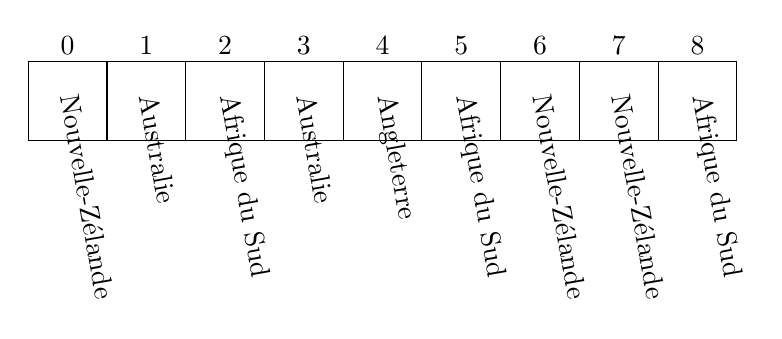
\begin{tikzpicture}
        \draw (0,0) grid (9,1);
        \foreach \x/\n in {0/Nouvelle-Zélande, 1/Australie, 2/Afrique du Sud, 3/Australie, 4/Angleterre, 5/Afrique du Sud, 6/Nouvelle-Zélande, 7/Nouvelle-Zélande, 8/Afrique du Sud}{
        \node[rotate=-80, anchor=west] at(0.5+\x, 0.7) {\n};
        \node at (0.5+\x, 1.2) {\x};
        }
    \end{tikzpicture}
\end{center}
\end{frame}
\begin{frame}[fragile]

\begin{center}
\begin{lstlisting}[language=Python , basicstyle=\ttfamily\small, xleftmargin=2em, xrightmargin=2em]
for equipe in gagnants:
    print(equipe)
\end{lstlisting}
\captionof{code}{Seconde méthode}
\label{CODE}
\end{center}  
\begin{center}
    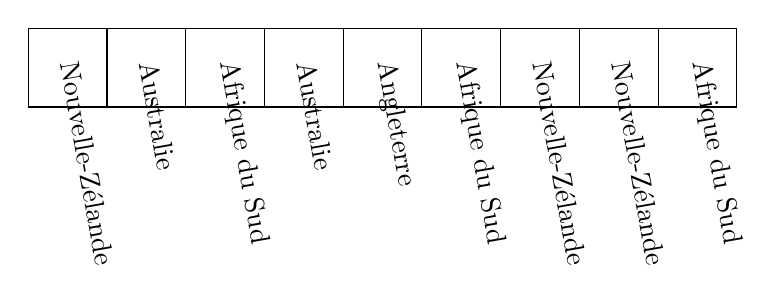
\begin{tikzpicture}
        \draw (0,0) grid (9,1);
        \foreach \x/\n in {0/Nouvelle-Zélande, 1/Australie, 2/Afrique du Sud, 3/Australie, 4/Angleterre, 5/Afrique du Sud, 6/Nouvelle-Zélande, 7/Nouvelle-Zélande, 8/Afrique du Sud}{
        \node[rotate=-80, anchor=west] at(0.5+\x, 0.7) {\n};
        }
    \end{tikzpicture}
\end{center}  
\begin{aretenir}[]
Il est possible d'\textbf{itérer} directement sur un tuple. À chaque tour de boucle la variable \textbf{\texttt{equipe}} contient l'élément suivant du tuple \textbf{\texttt{gagnants}}.
\end{aretenir}
\end{frame}
\begin{frame}
    \frametitle{}

    \begin{activite}
    \begin{enumerate}
        \item Écrire la fonction \textbf{\texttt{a\_gagne(palmares: tuple, equipe: str) $\rightarrow$ bool}} qui renvoie \textbf{\texttt{True}} si l'équipe passée en paramètre a déjà gagné la coupe du monde de rugby.
        \item Écrire la fonction \textbf{\texttt{nombre\_victoires(palmares: tuple, equipe: str) $\rightarrow$ int}} qui renvoie le nombre de victoires de \textbf{\texttt{equipe}}.
    \end{enumerate}
    \end{activite}

\end{frame}
\begin{frame}[fragile]
    \frametitle{Correction}

\begin{center}
\begin{lstlisting}[language=Python , basicstyle=\ttfamily\small, xleftmargin=1em, xrightmargin=0em]
def a_gagne(palmares: tuple, equipe: str) -> bool:
    """
    vérifie si l'équipe a déjà gagné
    """
    for i in range(len(palmares)):
        if palmares[i] == equipe:
            return True
    # on a parcouru tout le tuple
    return False
\end{lstlisting}
\captionof{code}{Création de la fonction}
\label{CODE}
\end{center}   
\begin{center}
\begin{lstlisting}[language=Python , basicstyle=\ttfamily\small, xleftmargin=2em, xrightmargin=2em]
>>> a_gagne(gagnants, "Nouvelle-Zélande")
True
\end{lstlisting}
\captionof{code}{Appel de la fonction}
\label{CODE}
\end{center}
\end{frame}
\begin{frame}[fragile]
    \frametitle{Correction}

\begin{center}
\begin{lstlisting}[language=Python , basicstyle=\ttfamily\small, xleftmargin=1em, xrightmargin=0em]
def a_gagne2(palmares: tuple, equipe: str) -> bool:
    """
    vérifie si l'équipe a déjà gagné
    """
    for e in palmares:
        if e == equipe:
            return True
    # on a parcouru tout le tuple
    return False
\end{lstlisting}
\captionof{code}{Deuxième méthode: itération sur le tuple}
\label{CODE}
\end{center}   

\end{frame}
\begin{frame}[fragile]
\begin{center}
\begin{lstlisting}[language=Python , basicstyle=\ttfamily\small, xleftmargin=0em, xrightmargin=-1em]
def nombre_victoires(palmares: tuple, equipe: str) -> int:
    """
    nombre de victoires de l'équipe
    """
    victoires = 0
    for i in range(len(palmares)):
        if palmares[i] == equipe:
            victoires += 1

    return victoires
\end{lstlisting}
\captionof{code}{Création de la fonction: Nombre de victoires}
\label{CODE}
\end{center}   
\begin{center}
\begin{lstlisting}[language=Python , basicstyle=\ttfamily\small, xleftmargin=2em, xrightmargin=2em]
>>> nombre_victoires(gagnants, "Australie")
2
\end{lstlisting}
\captionof{code}{Appel de la fonction}
\label{CODE}
\end{center}
\end{frame}
\begin{frame}[fragile]
\begin{center}
\begin{lstlisting}[language=Python , basicstyle=\ttfamily\small, xleftmargin=0em, xrightmargin=0em]
def nombre_victoires2(palmares: tuple, equipe: str) -> int:
    """
    nombre de victoires de l'équipe
    """
    victoires = 0
    for e in palmares:
        if e == equipe:
            victoires += 1

    return victoires
\end{lstlisting}
\captionof{code}{Seconde méthode}
\label{CODE}
\end{center}  
\end{frame}
\end{document}